\documentclass[border=10pt]{standalone}

\usepackage{tikz}
\usetikzlibrary{arrows.meta}

\tikzset{%
  >={Latex[width=2mm,length=2mm]},
  % Specifications for style of nodes:
  base/.style = {
    rectangle,
    rounded corners,
    % draw=black,
    % minimum width=4cm,
    % minimum height=2cm,
    text centered,
    font=\sffamily
  },
  %        process/.style = {base, minimum width=2.5cm, fill=orange!15,
  %                          font=\ttfamily},
  totEn/.style = {base, fill=orange!30},
  h_zero/.style = {base, fill=green!30, scale=0.8},
  h_scf/.style = {base, fill=gray!30, scale=0.8},
  module/.style = {base, fill=red!30, scale=0.6},
}

\begin{document}
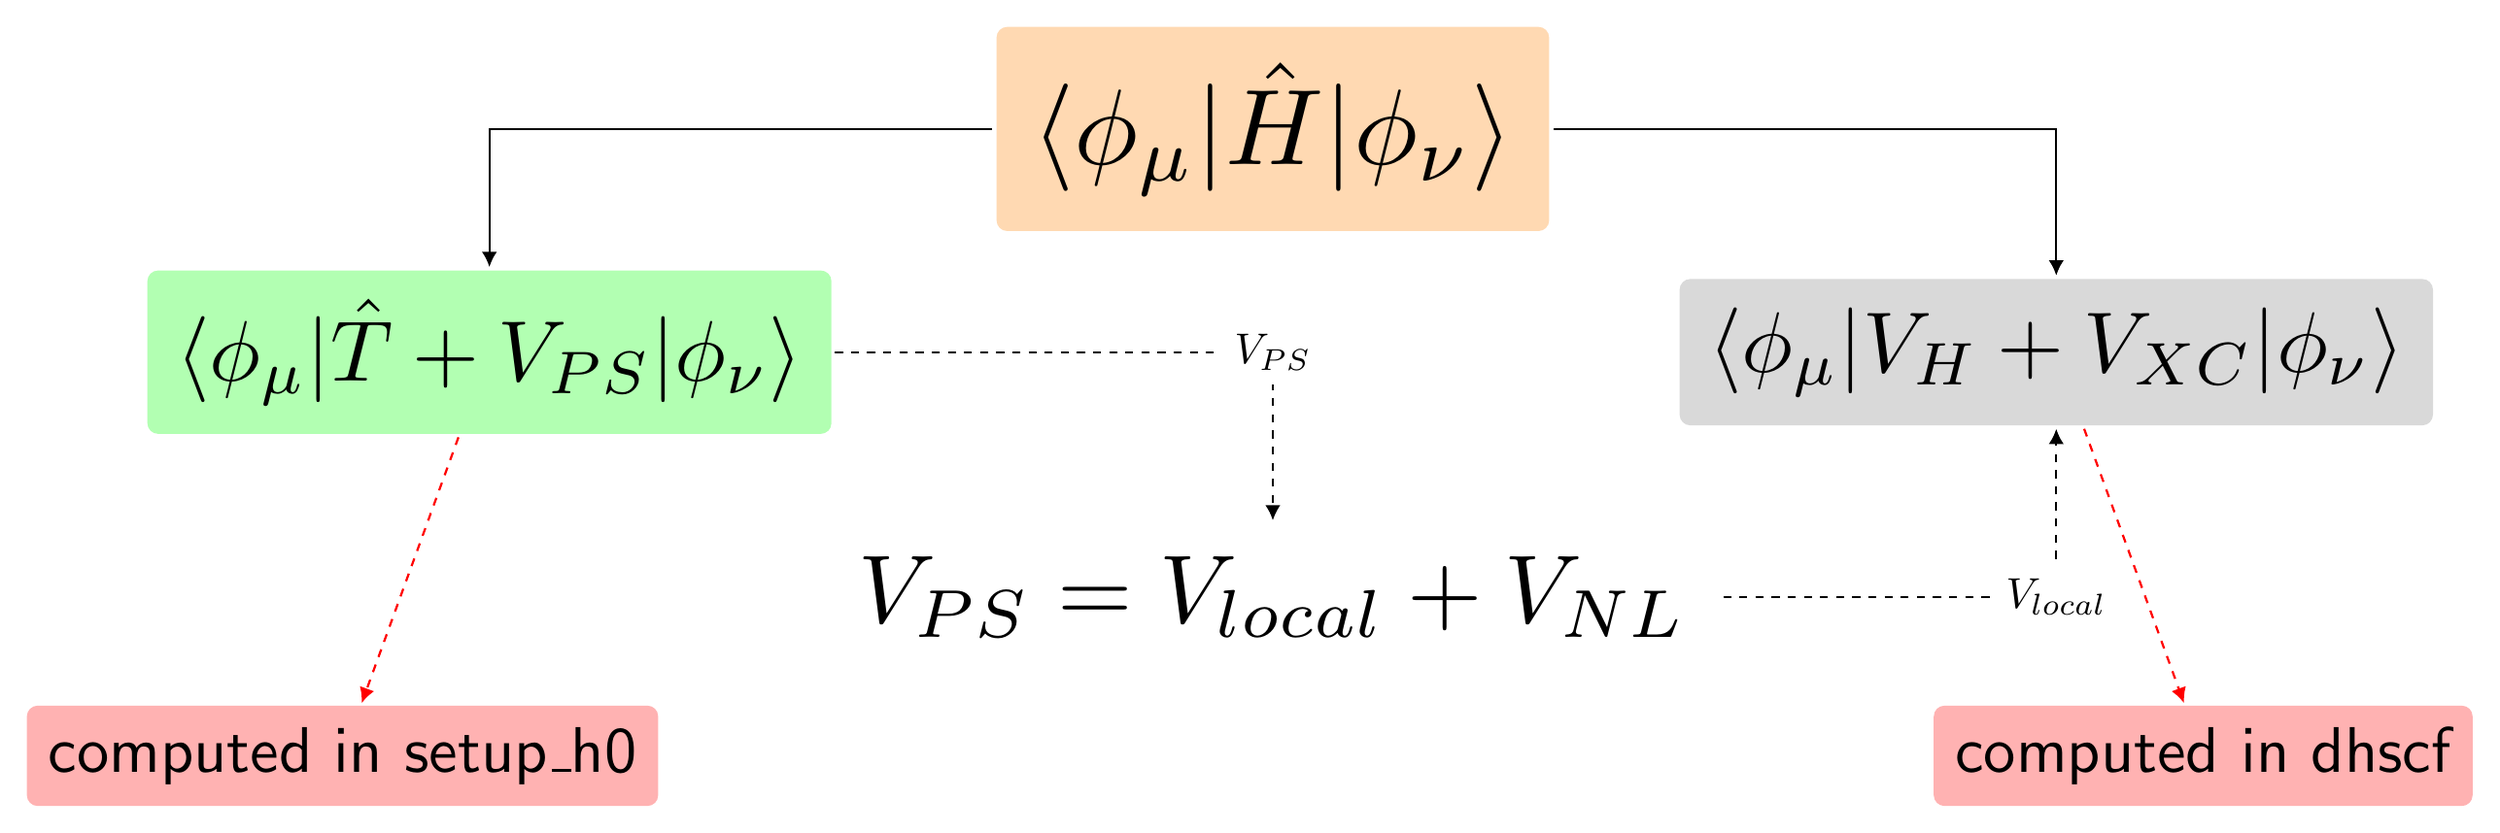
\begin{tikzpicture}[
  thick,
  scale=4.0,
  node distance=1.2cm,
  align=center,
  every node/.style={
    fill=white,
    font=\sffamily,
    transform shape
  },]
  % nodes
  \node (totEn)  [totEn]
  {\(\langle {\phi_{\mu} | \hat{H} | \phi_{\nu}} \rangle\)};
  \node (vps) [base, scale=0.9, below of=totEn, yshift=-0.5cm]
  {$V_{PS}=V_{local}+V_{NL}$};
  \node (h_zero) [h_zero, left of=vps, xshift=-2cm, yshift=1cm]
  {\(\langle {\phi_{\mu} | \hat{T} + V_{PS} | \phi_{\nu}} \rangle\)};
  \node (h_scf) [h_scf,  right of=vps, xshift=2cm, yshift=1cm]
  {\(\langle {\phi_{\mu} | V_{H} + V_{XC} | \phi_{\nu}} \rangle\)};
  \node (setup_h0) [module, below of=h_zero, xshift=-0.8cm, yshift=-1cm] {computed in setup\_h0};
  \node (setup_scf) [module, below of=h_scf, xshift=0.8cm, yshift=-1cm] {computed in dhscf};
  % lines
  \draw[->] (totEn) -| (h_zero);
  \draw[->] (totEn) -| (h_scf);
  \draw[->, dashed] (h_zero) -| node[scale=0.4](vps_ex){$V_{PS}$} (vps);
  \draw[->, dashed] (vps) -| node[scale=0.4](vlocal_ex){$V_{local}$}(h_scf);
  \draw[red, ->, dashed] (h_zero) -- (setup_h0);
  \draw[red, ->, dashed] (h_scf) -- (setup_scf);
\end{tikzpicture}
\end{document}
